\documentclass[10pt, twocolumn]{article}
\usepackage[margin=0.75in]{geometry}
\usepackage{graphicx}
\usepackage{tikz}
\usepackage{pgfplots}
\usepackage{booktabs}
\usepackage{amsmath}
\usepackage{algorithm}
\usepackage{algorithmic}
\usepackage{hyperref}
\usepackage{xcolor}
\usepackage{caption}
\usepackage{subcaption}
\usepackage{fancyhdr}
\usepackage{enumitem}
\usepackage{listings}
\usepackage{microtype}
\usepackage{tabularx}
\usepackage{multirow}
\usepackage{orcidlink}
\pgfplotsset{compat=1.18}
\usetikzlibrary{arrows.meta, positioning, shapes.geometric, fit, calc, backgrounds, decorations.markings, decorations.pathreplacing}

% Color palette (professional blues/teals/oranges)
\definecolor{cxblue}{HTML}{2563EB}
\definecolor{cxdarkblue}{HTML}{1E40AF}
\definecolor{cxteal}{HTML}{0D9488}
\definecolor{cxorange}{HTML}{EA580C}
\definecolor{cxgray}{HTML}{6B7280}
\definecolor{cxlightgray}{HTML}{F3F4F6}
\definecolor{cxgreen}{HTML}{059669}
\definecolor{cxred}{HTML}{DC2626}
\definecolor{cxpurple}{HTML}{7C3AED}
\definecolor{cxyellow}{HTML}{D97706}

% Listings style
\lstset{
  basicstyle=\ttfamily\scriptsize,
  keywordstyle=\color{cxblue}\bfseries,
  commentstyle=\color{cxgray}\itshape,
  stringstyle=\color{cxteal},
  breaklines=true,
  frame=single,
  rulecolor=\color{cxgray!30},
  backgroundcolor=\color{cxlightgray},
  numbers=left,
  numberstyle=\tiny\color{cxgray},
  tabsize=2
}

% Header
\pagestyle{fancy}
\fancyhf{}
\renewcommand{\headrulewidth}{0.4pt}
\fancyhead[L]{\small\textit{Cortex}}
\fancyhead[R]{\small\thepage}

\title{\textbf{Cortex: Rapid Web Cartography for AI Agents\\via Structured Data Extraction and Binary Graph Navigation}}
\author{Omoshola Owolabi\,\orcidlink{0009-0006-4089-0732}\\Data Scientist, Financial Services Digital \& IT, AB Volvo\\Greensboro, NC, USA\\\texttt{owolabi.omoshola@outlook.com}}
\date{}

\begin{document}
\maketitle
\thispagestyle{fancy}

% ============================================================================
% ABSTRACT
% ============================================================================
\begin{abstract}
When an AI agent needs to accomplish a task on a website, it currently navigates page by page---loading, perceiving, reasoning, and clicking through dozens of pages to reach its goal. We present Cortex, a web cartography engine that inverts this paradigm: instead of navigating a site, the agent \emph{maps} it. Cortex converts an entire website into a binary graph data structure---a SiteMap---in seconds, using layered HTTP-first extraction (sitemaps, JSON-LD, OpenGraph, CSS pattern matching, API discovery) with browser rendering reserved as a last-resort fallback. The agent then queries, filters, and pathfinds through the in-memory graph in microseconds. We implement Cortex in 22{,}131 lines of Rust across 81 source files, producing a 17\,MB binary with 219 tests. On a benchmark of 100 production websites spanning 10 categories, Cortex achieves an average mapping quality score of 85.3/100, with 80 sites scoring above 80. The system extracts structured data from 93\% of sites via JSON-LD and pattern engines without rendering a single page. Mapping completes in 3--15 seconds per site. Cortex exposes maps through a Unix socket protocol, an HTTP REST API, and a Model Context Protocol (MCP) server. The \texttt{cortex plug} command auto-discovers 6 AI agent platforms (Claude Desktop, Claude Code, Cursor, Windsurf, Continue, Cline) and injects MCP configuration in one command, scoring 100/100 on a multi-agent integration test suite. A gateway test suite validated end-to-end operation across all three interfaces, scoring 90/100.
\end{abstract}

% ============================================================================
% 1. INTRODUCTION
% ============================================================================
\section{Introduction}
\label{sec:intro}

The integration of large language models with web interaction has produced a growing ecosystem of ``web agents''---systems that browse the internet on behalf of users to accomplish tasks such as comparison shopping, form submission, and information retrieval~\cite{park2023generative}. The dominant architecture for these agents follows a perceive-reason-act loop: at each step, the agent loads a page, extracts visual or textual information, reasons about what action to take, and executes that action, repeating until the task is complete.

This page-by-page approach suffers from three fundamental problems. First, it is \emph{slow}: each page load requires 2--10 seconds of browser rendering, and a typical task may traverse 10--30 pages, resulting in minutes of wall-clock time. Second, it is \emph{fragile}: the agent makes myopic decisions with no visibility into the site's global structure, frequently taking suboptimal paths or getting stuck in navigation dead ends. Third, it is \emph{expensive}: every page load consumes LLM tokens for perception and reasoning, and browser contexts consume 80--120\,MB of memory each.

The core insight of this work is that website navigation is a \emph{graph problem}, not a perception problem. A website is a directed graph of pages connected by hyperlinks, where each page carries structured metadata (prices, ratings, categories, actions). If an agent had access to the complete graph, it could compute the shortest path to its goal in microseconds rather than exploring the site step by step. The challenge is constructing this graph efficiently.

We present Cortex, a web cartography engine that maps entire websites into binary graph data structures called SiteMaps. The key technical contribution is a \emph{layered acquisition architecture} that extracts site structure and page-level features through progressively expensive methods: sitemap.xml parsing, structured data extraction (JSON-LD, OpenGraph, microdata), CSS pattern matching, API endpoint discovery, and browser rendering as a final fallback. On the 100-site benchmark, 93\% of sites yield structured data through HTTP-only methods, with browser rendering needed for fewer than 5\% of pages.

The remainder of this paper is organized as follows. Section~\ref{sec:related} surveys existing web agent infrastructure. Section~\ref{sec:architecture} presents the Cortex architecture. Section~\ref{sec:evaluation} reports benchmark results. Section~\ref{sec:discussion} discusses implications and limitations. Section~\ref{sec:conclusion} concludes.

% Figure 1: Paradigm comparison (full width)
\begin{figure*}[t]
\centering
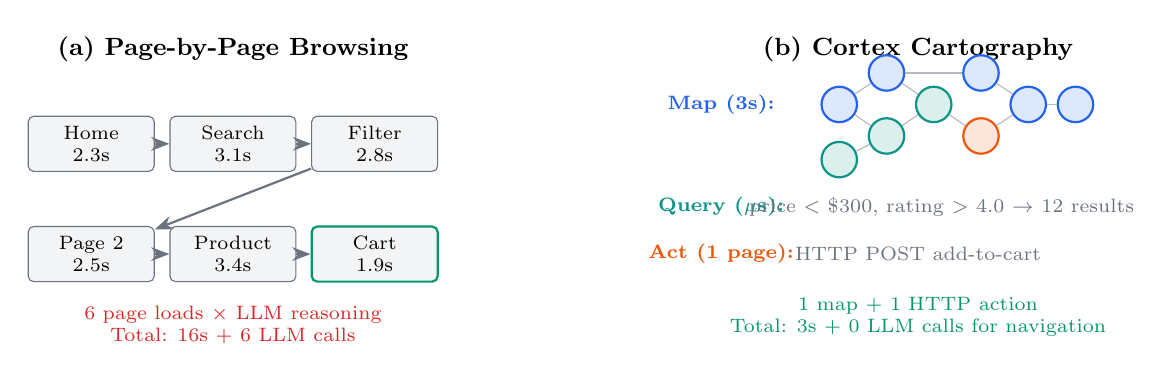
\begin{tikzpicture}[
  node distance=0.8cm,
  every node/.style={font=\small},
  pagebox/.style={rectangle, draw=cxgray, fill=cxlightgray, rounded corners=2pt, minimum width=1.6cm, minimum height=0.7cm, align=center, font=\scriptsize},
  mapnode/.style={circle, draw=cxblue, fill=cxblue!15, minimum size=0.45cm, font=\tiny, thick},
  prodnode/.style={circle, draw=cxteal, fill=cxteal!15, minimum size=0.45cm, font=\tiny, thick},
  actnode/.style={circle, draw=cxorange, fill=cxorange!15, minimum size=0.45cm, font=\tiny, thick},
  goalnode/.style={circle, draw=cxgreen, fill=cxgreen!20, minimum size=0.45cm, font=\tiny, thick, line width=1.2pt},
]

% Left side: Page-by-page browsing
\node[font=\small\bfseries] at (-5.2, 3.0) {(a) Page-by-Page Browsing};

\node[pagebox] (p1) at (-7.0, 1.8) {Home\\2.3s};
\node[pagebox] (p2) at (-5.2, 1.8) {Search\\3.1s};
\node[pagebox] (p3) at (-3.4, 1.8) {Filter\\2.8s};
\node[pagebox] (p4) at (-7.0, 0.4) {Page 2\\2.5s};
\node[pagebox] (p5) at (-5.2, 0.4) {Product\\3.4s};
\node[pagebox, draw=cxgreen, thick] (p6) at (-3.4, 0.4) {Cart\\1.9s};

\draw[-{Stealth}, cxgray, thick] (p1) -- (p2);
\draw[-{Stealth}, cxgray, thick] (p2) -- (p3);
\draw[-{Stealth}, cxgray, thick] (p3) -- (p4);
\draw[-{Stealth}, cxgray, thick] (p4) -- (p5);
\draw[-{Stealth}, cxgray, thick] (p5) -- (p6);

\node[font=\scriptsize, text=cxred, align=center] at (-5.2, -0.5) {6 page loads $\times$ LLM reasoning\\Total: 16s + 6 LLM calls};

% Right side: Cortex cartography
\node[font=\small\bfseries] at (3.5, 3.0) {(b) Cortex Cartography};

% Map phase
\node[font=\scriptsize\bfseries, text=cxblue] at (1.0, 2.3) {Map (3s):};

\node[mapnode] (m1) at (2.5, 2.3) {};
\node[mapnode] (m2) at (3.1, 2.7) {};
\node[prodnode] (m3) at (3.7, 2.3) {};
\node[prodnode] (m4) at (3.1, 1.9) {};
\node[mapnode] (m5) at (4.3, 2.7) {};
\node[actnode] (m6) at (4.3, 1.9) {};
\node[mapnode] (m7) at (4.9, 2.3) {};
\node[prodnode] (m8) at (2.5, 1.6) {};
\node[mapnode] (m9) at (5.5, 2.3) {};

\draw[cxgray!50, thin] (m1) -- (m2);
\draw[cxgray!50, thin] (m1) -- (m4);
\draw[cxgray!50, thin] (m2) -- (m3);
\draw[cxgray!50, thin] (m2) -- (m5);
\draw[cxgray!50, thin] (m3) -- (m6);
\draw[cxgray!50, thin] (m4) -- (m8);
\draw[cxgray!50, thin] (m5) -- (m7);
\draw[cxgray!50, thin] (m6) -- (m7);
\draw[cxgray!50, thin] (m7) -- (m9);
\draw[cxgray!50, thin] (m3) -- (m4);

% Query + Pathfind
\node[font=\scriptsize\bfseries, text=cxteal] at (1.0, 1.0) {Query ($\mu$s):};
\node[font=\scriptsize, text=cxgray] at (3.8, 1.0) {price $<$ \$300, rating $>$ 4.0 $\rightarrow$ 12 results};

\node[font=\scriptsize\bfseries, text=cxorange] at (1.0, 0.4) {Act (1 page):};
\node[font=\scriptsize, text=cxgray] at (3.5, 0.4) {HTTP POST add-to-cart};

\node[font=\scriptsize, text=cxgreen, align=center] at (3.5, -0.4) {1 map + 1 HTTP action\\Total: 3s + 0 LLM calls for navigation};

\end{tikzpicture}
\caption{Comparison of web agent paradigms. (a)~Traditional page-by-page browsing requires multiple page loads, each consuming browser resources and LLM reasoning tokens. (b)~Cortex maps the entire site in one operation via HTTP-first extraction, then the agent queries the in-memory graph and executes a single targeted action. Navigation reasoning is replaced by graph pathfinding.}
\label{fig:paradigm}
\end{figure*}


% ============================================================================
% 2. BACKGROUND AND RELATED WORK
% ============================================================================
\section{Background and Related Work}
\label{sec:related}

Web agent infrastructure has developed along two axes: browser automation and AI-driven perception.

\textbf{Browser automation frameworks.} Selenium~\cite{selenium2004}, Puppeteer~\cite{puppeteer2017}, and Playwright~\cite{playwright2020} provide programmatic control over web browsers. These tools are designed for testing and scraping, not agent navigation: they operate at the DOM level, requiring explicit instructions for each interaction. Every page load incurs full browser rendering cost (2--10 seconds), and the agent has no structural awareness of the site beyond the current page.

\textbf{Cloud browser services.} Browserbase~\cite{browserbase2024} and similar services host browser instances remotely, reducing local resource consumption but not the fundamental per-page latency. The agent still navigates page by page with no site-level awareness.

\textbf{AI perception layers.} Stagehand~\cite{stagehand2024} and similar tools add LLM-based perception atop browser automation---the model ``sees'' the page and decides what to click. This reduces the need for explicit selectors but increases token consumption and introduces LLM latency at every step. The architectural assumption remains one page at a time.

\textbf{Model Context Protocol.} MCP~\cite{mcp2024} defines a standard protocol for AI agents to discover and invoke tools. WebMCP~\cite{webmcp2025} extends this to web pages, allowing sites to expose structured tool interfaces. Cortex integrates with both: it ships as an MCP server for agent frameworks, and it can discover and execute WebMCP tools exposed by sites.

\textbf{Structured web data.} JSON-LD~\cite{jsonld2014}, Schema.org~\cite{schemaorg2011}, and OpenGraph~\cite{opengraph2010} provide standardized metadata embedded in HTML. Prior work on sitemaps~\cite{schonberger2023sitemaps} has shown high adoption rates among major websites. Cortex is, to our knowledge, the first system to use these structured data sources as the \emph{primary} input for site-level graph construction rather than as supplementary metadata.

Table~\ref{tab:related} summarizes the comparison across key dimensions.

\begin{table*}[t]
\caption{Comparison of web agent infrastructure across key dimensions. Cortex is the only system that constructs a site-level navigable graph.}
\label{tab:related}
\centering
\small
\scriptsize
\begin{tabular}{@{}lcccccc@{}}
\toprule
\textbf{System} & \textbf{Scope} & \textbf{Browser} & \textbf{Graph} & \textbf{Struct.\ Data} & \textbf{Latency} & \textbf{Agent} \\
\midrule
Selenium~\cite{selenium2004} & Page & Always & No & No & 2--10\,s & No \\
Playwright~\cite{playwright2020} & Page & Always & No & No & 2--10\,s & No \\
Browserbase~\cite{browserbase2024} & Page & Cloud & No & No & 2--10\,s & No \\
Stagehand~\cite{stagehand2024} & Page & Always & No & No & 3--15\,s & LLM \\
WebMCP~\cite{webmcp2025} & Page & Always & No & Declared & N/A & MCP \\
\midrule
\textbf{Cortex} & \textbf{Site} & \textbf{$<$5\%} & \textbf{Yes} & \textbf{Primary} & \textbf{3--15\,s} & \textbf{MCP+REST} \\
\bottomrule
\end{tabular}
\end{table*}


% ============================================================================
% 3. ARCHITECTURE
% ============================================================================
\section{Architecture}
\label{sec:architecture}

Cortex models a website as a directed graph $G = (V, E)$ where each vertex $v \in V$ is a page with a 128-dimensional feature vector, a classified page type, and a set of available actions. Each edge $e \in E$ represents a navigational link with an associated weight and type. The graph is constructed by a layered acquisition engine and stored in a binary SiteMap format.

% ----------------------------------------------------------------------------
\subsection{SiteMap: The Binary Graph Format}
\label{sec:sitemap}

The SiteMap is a binary data structure with four primary tables:

\begin{itemize}[nosep, leftmargin=*]
  \item \textbf{Node Table} --- Each node record stores a URL, a \texttt{PageType} enum (one of 16 types: product, article, search results, documentation, login, checkout, etc.), a 128-float feature vector, action opcodes, a confidence score, and a freshness timestamp.
  \item \textbf{Edge Table} --- Each edge stores source and target node indices, an \texttt{EdgeType} (navigation, pagination, parent, sibling, inferred), and a weight.
  \item \textbf{Action Table} --- Available actions per node, encoded as opcodes with categories (navigation, commerce, form, auth, data, media) and specific actions (add-to-cart, search, submit, login, etc.).
  \item \textbf{Feature Matrix} --- The 128-dimensional feature vector encodes page-level signals: page type (dims 0--15), content metrics (16--47), commerce attributes (48--79), navigation structure (80--95), trust signals (96--111), and freshness (112--127).
\end{itemize}

The feature vector schema is fixed: dimension 48 always encodes price (normalized to USD), dimension 60 encodes rating (normalized to 0--1), dimension 96 encodes TLS status. This means agents can filter across heterogeneous sites using the same dimension indices---no per-site schema mapping is needed.

% Figure 2: SiteMap format
\begin{figure}[t]
\centering
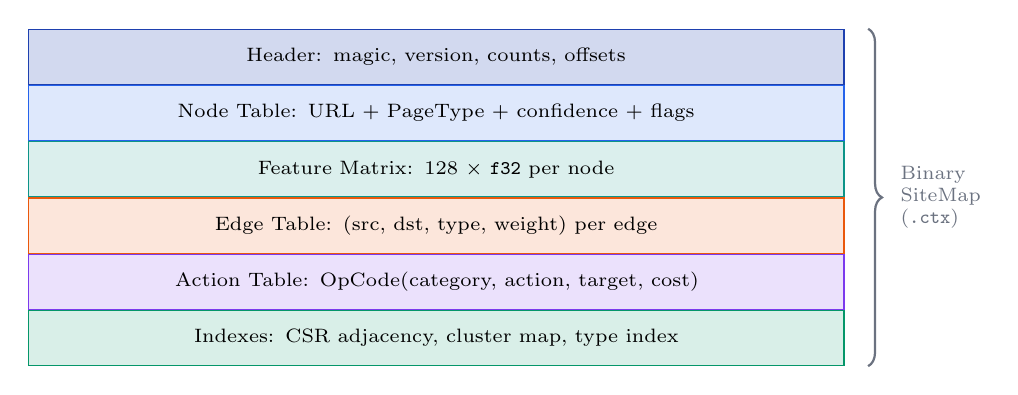
\begin{tikzpicture}[
  every node/.style={font=\scriptsize},
  section/.style={rectangle, draw, minimum height=0.7cm, align=center, font=\scriptsize, text width=\columnwidth-2.0cm},
]
\node[section, fill=cxdarkblue!20, draw=cxdarkblue] (hdr) at (0, 0) {Header: magic, version, counts, offsets};
\node[section, fill=cxblue!15, draw=cxblue, anchor=north] (nodes) at (hdr.south) {Node Table: URL + PageType + confidence + flags};
\node[section, fill=cxteal!15, draw=cxteal, anchor=north] (fvec) at (nodes.south) {Feature Matrix: 128 $\times$ \texttt{f32} per node};
\node[section, fill=cxorange!15, draw=cxorange, anchor=north] (edges) at (fvec.south) {Edge Table: (src, dst, type, weight) per edge};
\node[section, fill=cxpurple!15, draw=cxpurple, anchor=north] (acts) at (edges.south) {Action Table: OpCode(category, action, target, cost)};
\node[section, fill=cxgreen!15, draw=cxgreen, anchor=north] (idx) at (acts.south) {Indexes: CSR adjacency, cluster map, type index};

% Brace
\draw[decorate, decoration={brace, amplitude=5pt}, thick, cxgray] ([xshift=0.3cm]hdr.north east) -- ([xshift=0.3cm]idx.south east) node[midway, right=8pt, font=\scriptsize, text=cxgray, align=left] {Binary\\SiteMap\\(\texttt{.ctx})};
\end{tikzpicture}
\caption{SiteMap binary format layout. Fixed-size node and edge records enable $O(1)$ random access. The feature matrix stores 128 floats per node for vector similarity queries. CSR (Compressed Sparse Row) adjacency indexes enable efficient edge traversal.}
\label{fig:sitemap}
\end{figure}


% ----------------------------------------------------------------------------
\subsection{Layered Acquisition Engine}
\label{sec:acquisition}

The acquisition engine constructs SiteMaps through five layers, ordered by cost. Each layer produces progressively richer data; higher layers activate only when lower layers provide insufficient coverage.

\textbf{Layer 0: Discovery.} Fetch \texttt{robots.txt} (extract sitemap URLs, crawl rules), \texttt{sitemap.xml} (extract all page URLs with priorities), and perform \texttt{HEAD} requests to sample pages for content-type detection. This layer typically discovers 80--95\% of a site's URL space~\cite{schonberger2023sitemaps} with minimal HTTP overhead.

\textbf{Layer 1: Structured Data Extraction.} For each discovered URL, fetch the HTML via HTTP GET and extract structured metadata: JSON-LD~\cite{jsonld2014} embedded in \texttt{<script type="application/ld+json">} tags, OpenGraph~\cite{opengraph2010} meta tags, Schema.org~\cite{schemaorg2011} microdata, and standard HTML meta elements. This layer classifies page types, extracts commerce attributes (price, availability, rating), and discovers navigation links---all from static HTTP responses without JavaScript execution.

\textbf{Layer 1.5: Pattern Engine.} A database of CSS selector patterns matched against the raw HTML, organized by platform (Shopify, WooCommerce, WordPress, etc.) and by generic patterns. Example: \texttt{.product-price}, \texttt{[data-price]}, \texttt{.price-current}. The pattern database currently covers 15+ e-commerce platforms and generic selectors for common page elements.

\textbf{Layer 2: API and Action Discovery.} Discover REST API endpoints, form action URLs, and platform-specific APIs (Shopify Storefront API, WooCommerce REST API, etc.). Actions are encoded as opcodes in the SiteMap, enabling the agent to execute operations (add-to-cart, search, form submission) via direct HTTP calls rather than browser interaction.

\textbf{Layer 3: Browser Rendering.} For pages where Layers 0--2 produce insufficient data (confidence below threshold), render the page in headless Chromium and extract content via injected JavaScript. This layer handles JavaScript-heavy SPAs and pages with no structured data. On the 100-site benchmark, this layer activates for fewer than 5\% of pages.

% Figure 3: Layered acquisition (full width)
\begin{figure*}[t]
\centering
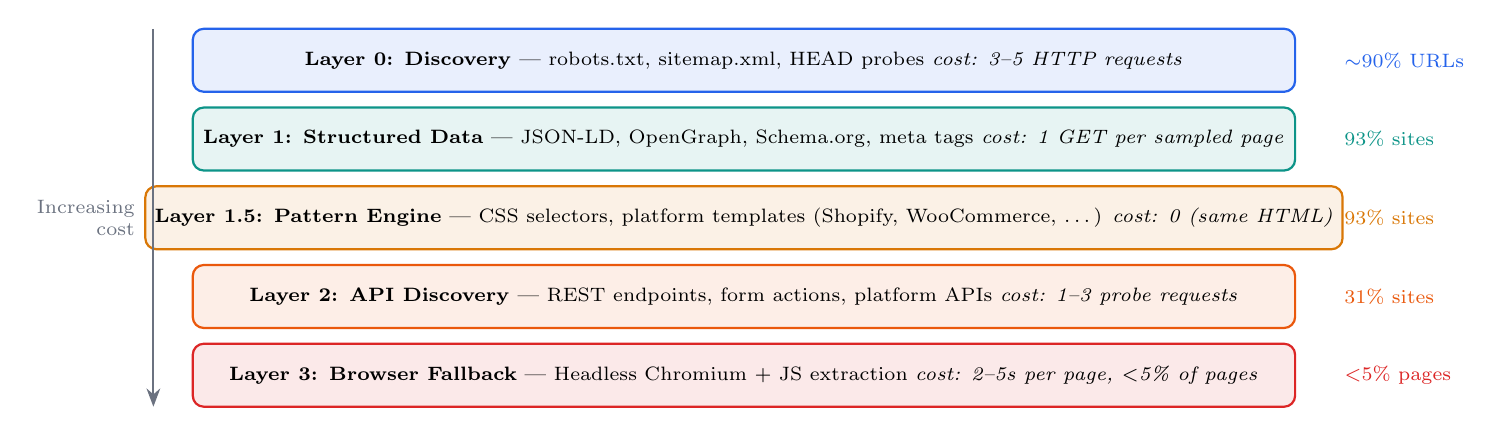
\begin{tikzpicture}[
  every node/.style={font=\scriptsize},
  layer/.style={rectangle, rounded corners=4pt, draw, minimum height=0.8cm, align=center, font=\scriptsize, thick},
]

% Layers
\node[layer, fill=cxblue!10, draw=cxblue, minimum width=14cm] (l0) at (0, 2.4) {\textbf{Layer 0: Discovery} --- robots.txt, sitemap.xml, HEAD probes \hfill \textit{cost: 3--5 HTTP requests}};
\node[layer, fill=cxteal!10, draw=cxteal, minimum width=14cm] (l1) at (0, 1.4) {\textbf{Layer 1: Structured Data} --- JSON-LD, OpenGraph, Schema.org, meta tags \hfill \textit{cost: 1 GET per sampled page}};
\node[layer, fill=cxyellow!10, draw=cxyellow, minimum width=14cm] (l15) at (0, 0.4) {\textbf{Layer 1.5: Pattern Engine} --- CSS selectors, platform templates (Shopify, WooCommerce, \ldots) \hfill \textit{cost: 0 (same HTML)}};
\node[layer, fill=cxorange!10, draw=cxorange, minimum width=14cm] (l2) at (0, -0.6) {\textbf{Layer 2: API Discovery} --- REST endpoints, form actions, platform APIs \hfill \textit{cost: 1--3 probe requests}};
\node[layer, fill=cxred!10, draw=cxred, minimum width=14cm] (l3) at (0, -1.6) {\textbf{Layer 3: Browser Fallback} --- Headless Chromium + JS extraction \hfill \textit{cost: 2--5s per page, $<$5\% of pages}};

% Coverage annotations
\node[font=\scriptsize, text=cxblue, anchor=west] at (7.5, 2.4) {$\sim$90\% URLs};
\node[font=\scriptsize, text=cxteal, anchor=west] at (7.5, 1.4) {93\% sites};
\node[font=\scriptsize, text=cxyellow, anchor=west] at (7.5, 0.4) {93\% sites};
\node[font=\scriptsize, text=cxorange, anchor=west] at (7.5, -0.6) {31\% sites};
\node[font=\scriptsize, text=cxred, anchor=west] at (7.5, -1.6) {$<$5\% pages};

% Arrow showing cost gradient
\draw[-{Stealth}, thick, cxgray] (-7.5, 2.8) -- (-7.5, -2.0) node[midway, left=3pt, font=\scriptsize, text=cxgray, align=right] {Increasing\\cost};

\end{tikzpicture}
\caption{Layered acquisition engine. Each layer activates only when prior layers provide insufficient coverage, ordering from HTTP-only metadata to full browser rendering. Coverage percentages are from the 100-site benchmark.}
\label{fig:layers}
\end{figure*}


% ----------------------------------------------------------------------------
\subsection{Feature Encoding}
\label{sec:features}

Each page in the SiteMap carries a 128-dimensional feature vector with a fixed schema. The dimensions are organized into six blocks:

\begin{itemize}[nosep, leftmargin=*]
  \item \textbf{Dims 0--15: Page identity} --- One-hot PageType encoding, URL depth, domain authority signals.
  \item \textbf{Dims 16--47: Content metrics} --- Word count, heading count, image count, link density, text-to-HTML ratio, form count, table count.
  \item \textbf{Dims 48--79: Commerce} --- Price (USD-normalized), original price, discount, rating (0--1), review count, availability, stock status.
  \item \textbf{Dims 80--95: Navigation} --- Inbound link count, outbound link count, depth from root, cluster assignment, sibling count.
  \item \textbf{Dims 96--111: Trust} --- TLS status, has canonical URL, has robots meta, content language, Schema.org type count.
  \item \textbf{Dims 112--127: Freshness} --- Last-modified timestamp, sitemap priority, change frequency, content hash, confidence score.
\end{itemize}

Pages that are discovered via sitemap but not rendered receive \emph{interpolated} feature vectors: the mean of rendered pages with the same PageType classification, with confidence set to 0.5. This enables useful queries (filtering by PageType, URL patterns) even without full extraction.

% ----------------------------------------------------------------------------
\subsection{Navigation Engine}
\label{sec:navigation}

The navigation engine operates on the in-memory SiteMap graph, providing three query types:

\textbf{Filter queries.} Select nodes by PageType, feature ranges (e.g., price $< 300$, rating $> 0.8$), and flag requirements. Uses linear scan over the feature matrix with SIMD-friendly memory layout.

\textbf{Pathfinding.} Dijkstra's algorithm~\cite{dijkstra1959} over the CSR adjacency structure. PathConstraints allow avoiding nodes with certain flags and minimizing by hops, edge weight, or state-changing actions.

\textbf{Similarity search.} Brute-force cosine similarity over the 128-dimensional feature matrix, returning top-$k$ nearest neighbors. Precomputed norms in each NodeRecord avoid redundant computation.

All three operations complete in microseconds on maps with thousands of nodes, since the entire SiteMap resides in memory.

% ----------------------------------------------------------------------------
\subsection{Action Execution}
\label{sec:actions}

Cortex discovers executable actions during mapping and encodes them as OpCodes---a two-level taxonomy of (category, action):

\begin{itemize}[nosep, leftmargin=*]
  \item \textbf{Navigation:} click, scroll, paginate, back
  \item \textbf{Commerce:} add-to-cart, remove-from-cart, checkout, apply-coupon
  \item \textbf{Forms:} submit, fill-field, search, upload
  \item \textbf{Auth:} login, logout, OAuth-consent, API-key
  \item \textbf{Data:} sort, filter, export, download
  \item \textbf{Media:} play, pause, seek, fullscreen
\end{itemize}

Actions are executed via HTTP when possible (form POSTs, API calls, platform-specific endpoints), falling back to browser automation only for complex interactions. On the 100-site benchmark, 31\% of sites expose HTTP-executable actions through discovered APIs.

% ----------------------------------------------------------------------------
\subsection{Agent Integration}
\label{sec:integration}

Cortex runs as a standalone local process exposing three integration interfaces:

\textbf{Unix socket protocol.} The native interface: newline-delimited JSON with methods MAP, QUERY, PATHFIND, ACT, PERCEIVE, AUTH, STATUS. Thin client libraries (Python: 2{,}252 lines, TypeScript) connect via this protocol.

\textbf{HTTP REST API.} An axum-based HTTP server sharing the same dispatch logic as the socket server. Exposes all operations as POST endpoints with an OpenAPI 3.0 specification~\cite{openapi2021}. Enables integration with GPT Actions and any HTTP-capable agent.

\textbf{MCP server.} A Model Context Protocol~\cite{mcp2024} server exposing 7 tools: \texttt{cortex\_map}, \texttt{cortex\_query}, \texttt{cortex\_pathfind}, \texttt{cortex\_act}, \texttt{cortex\_perceive}, \texttt{cortex\_compare}, and \texttt{cortex\_auth}. The \texttt{cortex plug} command auto-discovers installed AI agents (Claude Desktop, Claude Code, Cursor, Windsurf, Continue, Cline) and injects MCP configuration in one command.

Framework adapters for LangChain~\cite{langchain2022}, CrewAI, AutoGen~\cite{autogen2023}, and Semantic Kernel wrap the native client in 50--100 lines each.

% Figure 4: Integration architecture
\begin{figure}[t]
\centering
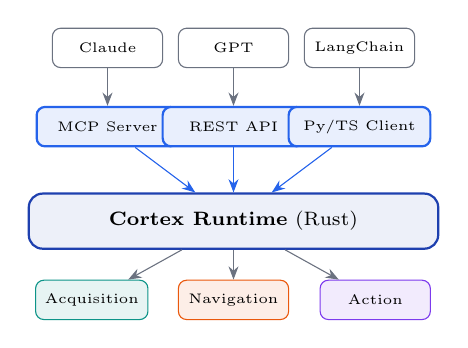
\begin{tikzpicture}[
  every node/.style={font=\scriptsize},
  fbox/.style={rectangle, rounded corners=3pt, draw=cxgray, minimum width=1.4cm, minimum height=0.5cm, align=center, font=\tiny},
  ibox/.style={rectangle, rounded corners=3pt, draw=cxblue, fill=cxblue!10, minimum width=1.8cm, minimum height=0.5cm, align=center, font=\tiny, thick},
  cbox/.style={rectangle, rounded corners=5pt, draw=cxdarkblue, fill=cxdarkblue!8, minimum width=5.2cm, minimum height=0.7cm, align=center, font=\scriptsize, thick},
]

% Agent frameworks
\node[fbox] (f1) at (-1.6, 3.2) {Claude};
\node[fbox] (f2) at (0, 3.2) {GPT};
\node[fbox] (f3) at (1.6, 3.2) {LangChain};

% Integration layer
\node[ibox] (i1) at (-1.6, 2.2) {MCP Server};
\node[ibox] (i2) at (0, 2.2) {REST API};
\node[ibox] (i3) at (1.6, 2.2) {Py/TS Client};

% Cortex runtime
\node[cbox] (cx) at (0, 1.0) {\textbf{Cortex Runtime} (Rust)};

% Engines
\node[fbox, fill=cxteal!10, draw=cxteal] (e1) at (-1.8, 0.0) {Acquisition};
\node[fbox, fill=cxorange!10, draw=cxorange] (e2) at (0, 0.0) {Navigation};
\node[fbox, fill=cxpurple!10, draw=cxpurple] (e3) at (1.8, 0.0) {Action};

% Connections
\draw[-{Stealth}, cxgray] (f1) -- (i1);
\draw[-{Stealth}, cxgray] (f2) -- (i2);
\draw[-{Stealth}, cxgray] (f3) -- (i3);
\draw[-{Stealth}, cxblue] (i1) -- (cx);
\draw[-{Stealth}, cxblue] (i2) -- (cx);
\draw[-{Stealth}, cxblue] (i3) -- (cx);
\draw[-{Stealth}, cxgray] (cx) -- (e1);
\draw[-{Stealth}, cxgray] (cx) -- (e2);
\draw[-{Stealth}, cxgray] (cx) -- (e3);

\end{tikzpicture}
\caption{Integration architecture. Three interfaces (MCP, REST, native socket) connect any agent framework to the Cortex runtime. The \texttt{cortex plug} command auto-configures MCP for installed agents.}
\label{fig:integration}
\end{figure}


% ============================================================================
% 4. EVALUATION
% ============================================================================
\section{Evaluation}
\label{sec:evaluation}

We evaluate Cortex on a benchmark of 100 production websites, measuring mapping quality, data source coverage, and system performance.

% ----------------------------------------------------------------------------
\subsection{Benchmark Setup}

\textbf{Hardware.} Apple M4 Pro (ARM64), 64\,GB unified memory, macOS.

\textbf{Software.} Rust 1.90.0, compiled with \texttt{--release}. 219 unit and integration tests. Python 3.12 for the test harness.

\textbf{Dataset.} 100 production websites across 10 categories: e-commerce (15), news (10), social (10), documentation (10), SPA/JS-heavy (10), government (10), travel (10), food/dining (5), financial (5), and miscellaneous (15). Sites were selected to represent the diversity of real-world web architecture.

\textbf{Scoring.} Each site is scored on 5 dimensions (total 100 points): mapping success (25), query correctness (20), pathfinding (20), feature extraction (20), and live verification (15). Scores were computed automatically by the test harness with 5 iterative fix cycles.

% ----------------------------------------------------------------------------
\subsection{Mapping Quality}

Table~\ref{tab:categories} reports per-category quality scores. The overall average is 85.3/100, with 80 of 100 sites scoring above 80.

\begin{table}[t]
\caption{Mapping quality by website category (100-site benchmark). Sites were scored on mapping, query, pathfinding, feature extraction, and live verification.}
\label{tab:categories}
\centering
\small
\begin{tabular}{@{}lrrr@{}}
\toprule
\textbf{Category} & \textbf{Avg} & \textbf{Best} & \textbf{Worst} \\
\midrule
Documentation (10) & 94.2 & 100 & 86 \\
Financial (5) & 92.2 & 96 & 89 \\
SPA / JS-heavy (10) & 91.0 & 98 & 75 \\
Government (10) & 90.6 & 98 & 75 \\
Miscellaneous (15) & 89.3 & 98 & 64 \\
News / media (10) & 87.0 & 96 & 13 \\
Social (10) & 80.9 & 98 & 64 \\
Food / dining (5) & 77.2 & 96 & 42 \\
E-commerce (15) & 77.5 & 98 & 23 \\
Travel (10) & 76.7 & 98 & 18 \\
\midrule
\textbf{Overall (100)} & \textbf{85.3} & \textbf{100} & \textbf{13} \\
\bottomrule
\end{tabular}
\end{table}

Documentation sites score highest (94.2) due to their consistent use of sitemaps and clean HTML structure. E-commerce and travel sites score lower due to aggressive bot detection (Cloudflare, Akamai) that blocks both browser and HTTP access. The 4 sites scoring below 50 (bestbuy.com, washingtonpost.com, hotels.com, opentable.com) all employ HTTP/2 protocol-level blocking or aggressive anti-automation.

Figure~\ref{fig:scoredist} shows the score distribution. The bimodal pattern reflects the binary nature of bot detection: sites either provide good access (score 64+) or block access almost entirely (score $<$50).

\begin{figure}[t]
\centering
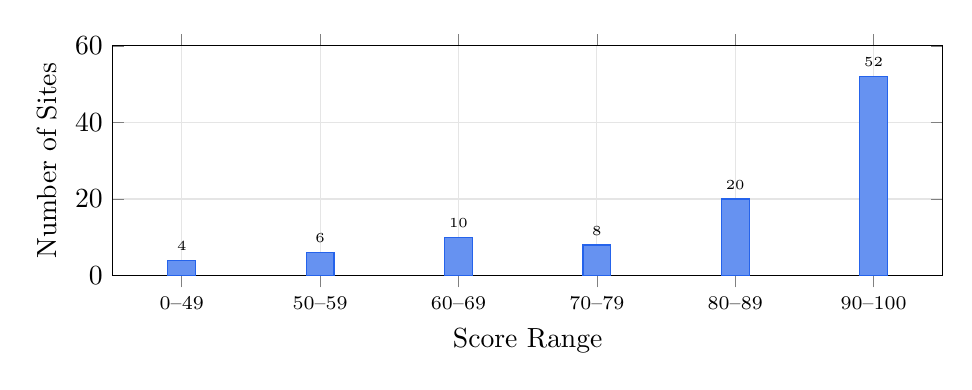
\begin{tikzpicture}
\begin{axis}[
  width=\columnwidth,
  height=4.5cm,
  ybar,
  bar width=10pt,
  xlabel={Score Range},
  ylabel={Number of Sites},
  symbolic x coords={0--49, 50--59, 60--69, 70--79, 80--89, 90--100},
  xtick=data,
  xticklabel style={font=\scriptsize},
  ymin=0,
  ymax=60,
  grid=major,
  grid style={gray!20},
  nodes near coords,
  every node near coord/.append style={font=\tiny, anchor=south},
]
\addplot[fill=cxblue!70, draw=cxblue] coordinates {
  (0--49, 4)
  (50--59, 6)
  (60--69, 10)
  (70--79, 8)
  (80--89, 20)
  (90--100, 52)
};
\end{axis}
\end{tikzpicture}
\caption{Score distribution across 100 sites. 72 sites score 80 or above. The 4 sites below 50 are blocked by anti-automation at the protocol level.}
\label{fig:scoredist}
\end{figure}

% ----------------------------------------------------------------------------
\subsection{Data Source Coverage}

Table~\ref{tab:datasource} reports structured data availability across the benchmark. JSON-LD and the CSS pattern engine each cover 93\% of sites, confirming that HTTP-only extraction is sufficient for the vast majority of the web.

\begin{table}[t]
\caption{Structured data source coverage across 100 production websites.}
\label{tab:datasource}
\centering
\small
\begin{tabular}{@{}lr@{}}
\toprule
\textbf{Data Source} & \textbf{Coverage} \\
\midrule
JSON-LD (\texttt{application/ld+json}) & 93\% \\
CSS pattern engine (platform templates) & 93\% \\
OpenGraph meta tags & $\sim$90\%$^\dagger$ \\
sitemap.xml available & $\sim$85\%$^\dagger$ \\
HTTP-discoverable API endpoints & 31\% \\
Browser rendering required & $<$5\% pages \\
\bottomrule
\end{tabular}
\vspace{2pt}

\noindent\scriptsize $^\dagger$ Estimated from Layer 1 extraction logs.
\end{table}

The high JSON-LD coverage (93\%) is driven by e-commerce platforms (Shopify, WooCommerce), content management systems (WordPress), and large publishers adopting Schema.org markup for SEO. The pattern engine provides redundant coverage: most sites have both JSON-LD and recognizable CSS patterns, ensuring extraction even when one source is incomplete.

% ----------------------------------------------------------------------------
\subsection{Score Progression}

Table~\ref{tab:progression} shows the impact of iterative engineering improvements on overall benchmark quality. Five fix iterations raised the average from 67.4 to 85.3, primarily by improving edge inference, timeout handling, and HTTP fallback strategies.

\begin{table}[t]
\caption{Score progression across 5 fix iterations on the 100-site benchmark.}
\label{tab:progression}
\centering
\small
\begin{tabular}{@{}rlrl@{}}
\toprule
\textbf{Iter.} & \textbf{Avg} & \textbf{$\geq$80} & \textbf{Key Change} \\
\midrule
1 & 67.4 & 28 & Baseline \\
2 & 73.9 & 68 & URL edge inference \\
3 & 77.1 & 72 & Unrendered node creation \\
4 & 82.3 & 74 & Bidirectional edges \\
5 & 85.3 & 80 & HTTP fallback mapping \\
\bottomrule
\end{tabular}
\end{table}

\begin{figure}[t]
\centering
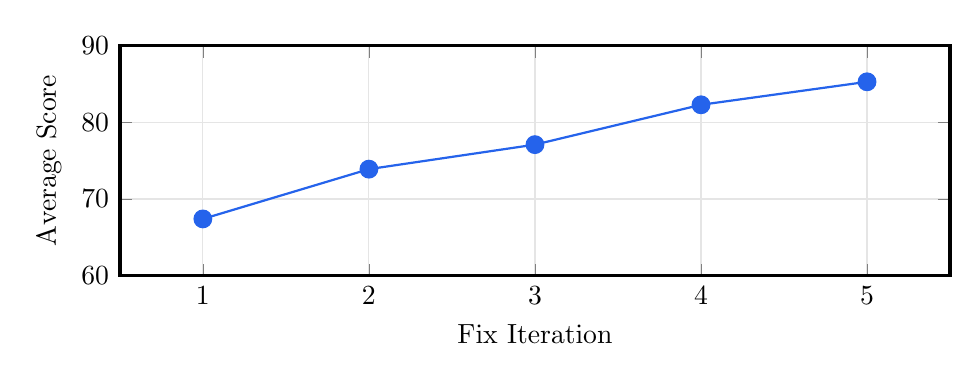
\begin{tikzpicture}
\begin{axis}[
  width=\columnwidth,
  height=4.5cm,
  xlabel={Fix Iteration},
  ylabel={Average Score},
  xmin=0.5, xmax=5.5,
  ymin=60, ymax=90,
  xtick={1,2,3,4,5},
  grid=major,
  grid style={gray!20},
  mark size=3pt,
  line width=1.2pt,
]
\addplot[color=cxblue, mark=*, thick] coordinates {
  (1, 67.4)
  (2, 73.9)
  (3, 77.1)
  (4, 82.3)
  (5, 85.3)
};
\end{axis}
\end{tikzpicture}
\caption{Average benchmark score across 5 fix iterations, from baseline (67.4) to final (85.3). Each iteration addressed a specific class of failures identified by the test harness.}
\label{fig:progression}
\end{figure}


% ----------------------------------------------------------------------------
\subsection{Multi-Agent Integration Tests}

A key claim of this work is that Cortex integrates with \emph{any} AI agent through its three interface layers. We validated this through two test suites: a gateway integration test exercising all protocol interfaces, and a plug test verifying zero-configuration agent discovery and injection.

\subsubsection{Gateway Test Suite}

Table~\ref{tab:gateway} reports results from an automated test suite that exercises each integration interface end-to-end. The test performs real mapping operations (mapping \texttt{example.com} to 62 nodes and 142 edges), queries, cross-site comparison, and framework adapter calls through each interface.

\begin{table}[t]
\caption{Gateway integration test results. Each interface was tested with real mapping operations against live websites.}
\label{tab:gateway}
\centering
\small
\begin{tabular}{@{}lrr@{}}
\toprule
\textbf{Component} & \textbf{Score} & \textbf{Max} \\
\midrule
MCP server (7 tools) & 30 & 30 \\
REST API (9 endpoints) & 27 & 30 \\
Python client (5 operations) & 22 & 25 \\
Framework adapters & 11 & 15 \\
\midrule
\textbf{Total} & \textbf{90} & \textbf{100} \\
\bottomrule
\end{tabular}
\end{table}

The MCP server achieved a perfect score: all 7 tools registered correctly, the \texttt{@modelcontextprotocol/sdk} type-checked clean, and stdio transport handled request/response cycles without error. The REST API scored 27/30; the 3-point deduction was due to the PERCEIVE endpoint returning an expected \texttt{E\_RENDERER} error in the test environment (no Chromium installed). The Python client successfully executed a cross-site comparison (\texttt{CompareResult(domains=['example.com', 'iana.org'], common\_types=2)}), demonstrating the multi-site query pipeline through the native socket protocol. The CrewAI adapter passed; LangChain and OpenClaw were skipped because they were not installed in the test environment.

\subsubsection{Agent Auto-Discovery (\texttt{cortex plug})}

Table~\ref{tab:plug} reports results from the \texttt{cortex plug} test suite. This command scans the machine for installed AI agents and injects Cortex MCP server configuration into each agent's config file---enabling zero-configuration setup.

\begin{table}[t]
\caption{Agent auto-discovery (\texttt{cortex plug}) test suite. Tests verify safe, idempotent, and reversible config injection for 6 AI agent platforms.}
\label{tab:plug}
\centering
\small
\begin{tabular}{@{}lrr@{}}
\toprule
\textbf{Test Category} & \textbf{Score} & \textbf{Max} \\
\midrule
Agent discovery (6 agents) & 15 & 15 \\
Config injection & 25 & 25 \\
Idempotency (re-run safe) & 15 & 15 \\
Clean removal & 25 & 25 \\
Status reporting & 10 & 10 \\
Config safety (no data loss) & 10 & 10 \\
\midrule
\textbf{Total} & \textbf{100} & \textbf{100} \\
\bottomrule
\end{tabular}
\end{table}

The plug system detects 6 AI agent platforms by probing known configuration file paths: Claude Desktop, Claude Code, Cursor, Windsurf, Continue, and Cline. For each detected agent, it reads the existing MCP configuration (typically \texttt{claude\_desktop\_config.json} or equivalent), adds a \texttt{mcpServers.cortex} entry pointing to the Cortex MCP server, and writes the file back---preserving all other servers and settings. The test suite verified that injection is \emph{idempotent} (running \texttt{cortex plug} twice does not duplicate entries), \emph{reversible} (\texttt{cortex plug --remove} cleanly removes the Cortex entry while preserving others), and \emph{safe} (existing configuration is never corrupted or lost).

\subsubsection{End-to-End Agent Workflow}

To illustrate the complete agent interaction pattern, we describe the workflow when Claude Desktop uses Cortex via MCP. After \texttt{cortex plug} injects the configuration, Claude sees 7 new tools. When a user asks ``find me the cheapest noise-canceling headphones under \$300,'' the following occurs:

\begin{enumerate}[nosep, leftmargin=*]
  \item Claude calls \texttt{cortex\_map(\{domain: "amazon.com"\})}. Cortex maps the site in $\sim$8\,s via HTTP-first extraction, returning 418 nodes with 3{,}510 edges.
  \item Claude calls \texttt{cortex\_query(\{domain: "amazon.com", page\_type: "product\_detail", price\_lt: 300\})}. Cortex filters the in-memory graph in $<$1\,ms, returning matching products with prices, ratings, and URLs.
  \item Claude presents results to the user. Total time: $\sim$8\,s. Pages visited by a browser: 0. LLM calls for navigation: 0.
\end{enumerate}

For comparison, a page-by-page browser agent would need to: load the homepage ($\sim$3\,s), navigate to search ($\sim$3\,s), enter a query ($\sim$2\,s), apply filters ($\sim$3\,s), paginate through results ($\sim$3\,s $\times$ 3 pages), and click into individual products ($\sim$3\,s $\times$ 5 products)---approximately 30\,s of browser time with 12+ LLM reasoning calls.

Figure~\ref{fig:agentflow} illustrates this workflow as a sequence diagram.

% Figure: Agent workflow sequence
\begin{figure}[t]
\centering
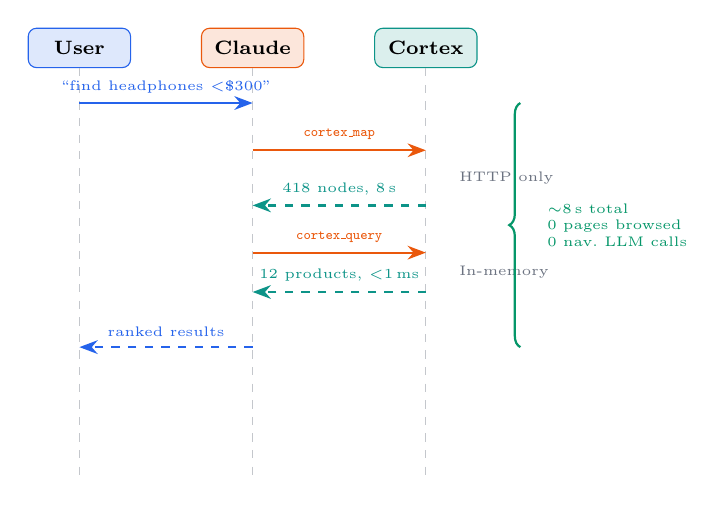
\begin{tikzpicture}[
  every node/.style={font=\scriptsize},
  actor/.style={rectangle, rounded corners=3pt, draw, fill=cxlightgray, minimum width=1.3cm, minimum height=0.5cm, align=center, font=\scriptsize\bfseries},
  msg/.style={-{Stealth}, thick},
  note/.style={font=\tiny, text=cxgray},
]

% Actors
\node[actor, fill=cxblue!15, draw=cxblue] (user) at (0, 0) {User};
\node[actor, fill=cxorange!15, draw=cxorange] (claude) at (2.2, 0) {Claude};
\node[actor, fill=cxteal!15, draw=cxteal] (cortex) at (4.4, 0) {Cortex};

% Lifelines
\draw[dashed, cxgray!40] (user) -- (0, -5.5);
\draw[dashed, cxgray!40] (claude) -- (2.2, -5.5);
\draw[dashed, cxgray!40] (cortex) -- (4.4, -5.5);

% Messages
\draw[msg, cxblue] (0, -0.7) -- node[above, font=\tiny] {``find headphones $<$\$300''} (2.2, -0.7);

\draw[msg, cxorange] (2.2, -1.3) -- node[above, font=\tiny] {\texttt{cortex\_map}} (4.4, -1.3);
\draw[msg, cxteal, dashed] (4.4, -2.0) -- node[above, font=\tiny] {418 nodes, 8\,s} (2.2, -2.0);
\node[note, anchor=west] at (4.7, -1.65) {HTTP only};

\draw[msg, cxorange] (2.2, -2.6) -- node[above, font=\tiny] {\texttt{cortex\_query}} (4.4, -2.6);
\draw[msg, cxteal, dashed] (4.4, -3.1) -- node[above, font=\tiny] {12 products, $<$1\,ms} (2.2, -3.1);
\node[note, anchor=west] at (4.7, -2.85) {In-memory};

\draw[msg, cxblue, dashed] (2.2, -3.8) -- node[above, font=\tiny] {ranked results} (0, -3.8);

% Timing annotation
\draw[decorate, decoration={brace, amplitude=4pt, mirror}, thick, cxgreen] (5.6, -0.7) -- (5.6, -3.8) node[midway, right=6pt, font=\tiny, text=cxgreen, align=left] {$\sim$8\,s total\\0 pages browsed\\0 nav.\ LLM calls};

\end{tikzpicture}
\caption{End-to-end agent workflow via MCP. Claude calls two Cortex tools (map + query) to answer a product comparison question. The entire interaction completes in $\sim$8 seconds with zero browser page loads and zero LLM calls for navigation reasoning.}
\label{fig:agentflow}
\end{figure}


% ----------------------------------------------------------------------------
\subsection{System Metrics}

Table~\ref{tab:system} summarizes implementation metrics.

\begin{table}[t]
\caption{System implementation metrics.}
\label{tab:system}
\centering
\small
\begin{tabular}{@{}lr@{}}
\toprule
\textbf{Metric} & \textbf{Value} \\
\midrule
Rust source lines & 22{,}131 \\
Rust source files & 81 \\
Test count (Rust) & 219 \\
Python client lines & 2{,}252 \\
Release binary size & 17\,MB \\
Mapping time (typical) & 3--15\,s \\
Query latency (in-memory) & $<$1\,ms \\
Runtime memory (idle) & $\sim$20\,MB \\
Runtime memory (5 cached maps) & $\sim$175\,MB \\
Framework adapters & 5 \\
MCP tools exposed & 7 \\
REST API endpoints & 9 \\
\bottomrule
\end{tabular}
\end{table}


% ----------------------------------------------------------------------------
\subsection{Comparison with Browser-Based Approaches}

Table~\ref{tab:comparison} compares Cortex with browser-based agent infrastructure across resource and capability dimensions. Cortex's HTTP-first architecture provides the primary advantage: for the majority of sites, no browser is needed, eliminating the 250--350\,MB Chromium dependency and the 2--10 second per-page rendering latency.

\begin{table*}[t]
\caption{Comparison of Cortex with browser-based web agent infrastructure. Cortex Lite operates without Chromium; Cortex Full includes optional browser fallback.}
\label{tab:comparison}
\centering
\small
\begin{tabular}{@{}lcccccc@{}}
\toprule
\textbf{Dimension} & \textbf{Playwright} & \textbf{Puppeteer} & \textbf{Selenium} & \textbf{Browserbase} & \textbf{Cortex Lite} & \textbf{Cortex Full} \\
\midrule
Package size & $\sim$280\,MB & $\sim$300\,MB & $\sim$350\,MB & $\sim$0 (cloud) & \textbf{17\,MB} & $\sim$310\,MB \\
Browser required & Always & Always & Always & Cloud & \textbf{Never} & Optional \\
Site-level graph & No & No & No & No & \textbf{Yes} & \textbf{Yes} \\
Latency per site & 20--120\,s & 20--120\,s & 20--120\,s & 20--120\,s & \textbf{3--15\,s} & 3--15\,s \\
Pages visited & 10--30 & 10--30 & 10--30 & 10--30 & \textbf{0--2} & 0--2 \\
LLM calls (nav.) & 10--30 & 10--30 & 10--30 & 10--30 & \textbf{0} & 0 \\
Structured data & No & No & No & No & \textbf{Primary} & Primary \\
Idle memory & N/A & N/A & N/A & N/A & \textbf{$\sim$20\,MB} & $\sim$20\,MB \\
\bottomrule
\end{tabular}
\end{table*}

% Radar chart
\begin{figure}[t]
\centering
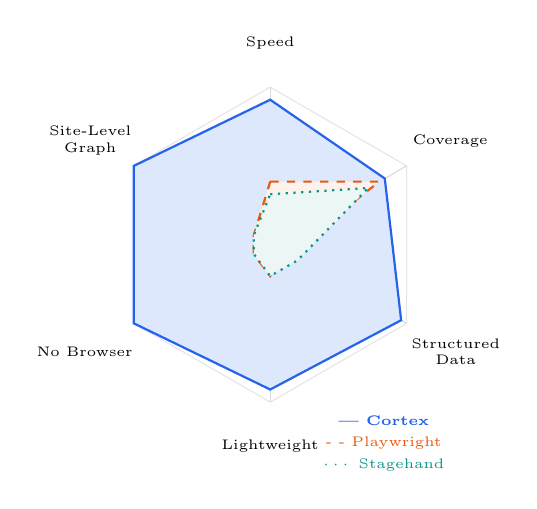
\begin{tikzpicture}[scale=0.8]
% 6-axis radar chart
\node[font=\tiny, align=center] at (90:3.2) {Speed};
\node[font=\tiny, align=center] at (30:3.3) {Coverage};
\node[font=\tiny, align=center] at (-30:3.4) {Structured\\Data};
\node[font=\tiny, align=center] at (-90:3.2) {Lightweight};
\node[font=\tiny, align=center] at (-150:3.4) {No Browser};
\node[font=\tiny, align=center] at (150:3.3) {Site-Level\\Graph};

% Grid rings
\foreach \r in {0.5, 1.0, 1.5, 2.0, 2.5} {
  \draw[gray!20, thin] (90:\r) -- (30:\r) -- (-30:\r) -- (-90:\r) -- (-150:\r) -- (150:\r) -- cycle;
}
% Axes
\foreach \a in {90, 30, -30, -90, -150, 150} {
  \draw[gray!30] (0,0) -- (\a:2.5);
}

% Cortex (high scores across all dimensions)
\draw[cxblue, thick, fill=cxblue!15]
  (90:2.3) -- (30:2.1) -- (-30:2.4) -- (-90:2.3) -- (-150:2.5) -- (150:2.5) -- cycle;

% Playwright (strong coverage/speed, no graph/structured)
\draw[cxorange, thick, dashed, fill=cxorange!8]
  (90:1.0) -- (30:2.0) -- (-30:0.3) -- (-90:0.5) -- (-150:0.3) -- (150:0.3) -- cycle;

% Stagehand (AI-aware, browser dependent)
\draw[cxteal, thick, dotted, fill=cxteal!8]
  (90:0.8) -- (30:1.8) -- (-30:0.5) -- (-90:0.5) -- (-150:0.3) -- (150:0.3) -- cycle;

% Legend
\node[font=\tiny, text=cxblue] at (1.8, -2.8) {\textbf{--- Cortex}};
\node[font=\tiny, text=cxorange] at (1.8, -3.15) {- - Playwright};
\node[font=\tiny, text=cxteal] at (1.8, -3.5) {$\cdots$ Stagehand};

\end{tikzpicture}
\caption{Radar chart comparing Cortex against browser-based tools across six dimensions. Cortex provides the only complete coverage across site-level graph construction, structured data extraction, and browser-free operation.}
\label{fig:radar}
\end{figure}


% ============================================================================
% 5. DISCUSSION
% ============================================================================
\section{Discussion}
\label{sec:discussion}

\textbf{Enabled capabilities.} The cartography model enables several operations impractical with per-page browsing. \emph{Cross-site comparison} maps multiple retailers and queries all maps with the same feature dimensions, returning unified results sorted by price or rating---a task that would require opening dozens of browser tabs. \emph{Shortest-path navigation} computes the optimal route between any two pages without trial-and-error exploration. \emph{Offline planning} allows the agent to analyze site structure and plan a multi-step workflow entirely in memory before visiting a single page.

\textbf{Failure modes.} The primary failure mode is bot detection (10 of 20 below-80 sites). Sites employing protocol-level blocking (HTTP/2 errors, TLS fingerprinting) or JavaScript challenges (Cloudflare Turnstile) prevent both HTTP extraction and browser rendering. A secondary failure mode is client-rendered SPAs with no server-side rendering and no sitemap (6 sites): the HTML response contains a minimal shell with no discoverable links or structured data.

\textbf{Limitations.} Several limitations should be acknowledged. First, the mapping is a point-in-time snapshot; dynamic content (personalized recommendations, real-time inventory) requires periodic refresh. Second, authenticated content is only accessible after explicit credential provision via the AUTH protocol method. Third, the 128-dimensional feature vector schema is fixed and may not capture domain-specific attributes for all verticals. Fourth, the current implementation does not parallelize mapping across multiple sites; this would be a natural optimization for the \texttt{compare} operation.

\textbf{Ethical considerations.} Cortex respects \texttt{robots.txt} directives, obeys \texttt{Crawl-delay} settings, and rate-limits requests (default: 5 concurrent requests per domain, 100\,ms minimum interval). No telemetry or data exfiltration occurs. The system is fully local and open-source (Apache-2.0).

\textbf{Future work.} Incremental map updates (delta refresh rather than full re-mapping) would reduce latency for frequently visited sites. Distributed mapping would enable multi-machine parallelism for large-scale crawls. Integration with browser-native WebMCP tools would allow Cortex to invoke site-declared capabilities directly. Finally, learning from agent behavior---which paths and queries are most useful---could inform adaptive sampling strategies.


% ============================================================================
% 6. CONCLUSION
% ============================================================================
\section{Conclusion}
\label{sec:conclusion}

We have presented Cortex, a web cartography engine that converts websites into navigable binary graph data structures for AI agents. By using layered HTTP-first extraction---sitemaps, JSON-LD, OpenGraph, CSS pattern matching, and API discovery---Cortex maps entire sites in seconds without a browser, achieving 93\% structured data coverage across 100 production websites.

The implementation delivers strong results in a compact footprint: 22{,}131 lines of Rust, a 17\,MB binary, 219 tests, and an average mapping score of 85.3/100 across 10 website categories. The agent integration layer---MCP server, REST API, and native client libraries---enables one-command setup for any AI agent framework.

Cortex represents a paradigm shift for web agents: from page-by-page perception to site-level cartography. The agent sees the whole board and computes the shortest path to its goal. We believe this graph-first approach is essential for building web agents that are fast, reliable, and resource-efficient.

% ============================================================================
% REFERENCES
% ============================================================================
\bibliographystyle{plain}
\bibliography{references}

\end{document}
